\subsection{Hidden Markov Models}

HMMs are common statistical models used to describe time series that exhibit state-switching behavior. An HMM models an observed sequence of length $T$, $\bfY = \{Y_t\}_{t=1}^T$, together with an unobserved (or  ``hidden") sequence $\bfX = \{X_t\}_{t=1}^T$. The hidden sequence $\bfX$ is a Markov chain, and each observation $Y_t$ is a random variable, where $Y_t$ given all other observations $\bfY \setminus \{Y_t\}$ and hidden states $\bfX$ depends only on $X_t$. While the sample space of $\bfX$ is general, we assume $X_t \in \{1,\ldots,N\}$ for some finite $N$. The unconditional distribution of $X_1$ is denoted by the row-vector
%
\begin{equation}
    \bfdelta = \begin{pmatrix} \delta^{(1)} & \cdots & \delta^{(N)} \end{pmatrix},
\end{equation}
%
where $\delta^{(i)} = \bbP(X_1 = i)$. Further, the distribution of $X_t$ for $t > 1$ conditioned on $X_{t-1}$ is denoted by an $N$-by-$N$ transition probability matrix 
%
\begin{equation}
    \bfGamma_t = \begin{pmatrix} 
    \Gamma_t^{(1,1)} & \cdots & \Gamma_t^{(1,N)} \\
    \vdots & \ddots & \vdots \\
    \Gamma_t^{(N,1)} & \cdots & \Gamma_t^{(N,N)} \\
    \end{pmatrix},
\end{equation}
%
where $\Gamma_t^{(i,j)} = \bbP(X_t = j \mid X_{t-1} = i)$. %Our methods apply to transition probability matrices that depend upon time, but for ease of presentation
For simplicity, we assume that $\bfGamma_t$ does not change over time (i.e. $\bfGamma_t = \bfGamma$ for all $t$) unless stated otherwise. 

%We assume that the distribution of an observation $Y_t$ conditioned on the corresponding hidden state $X_t$ does not depend upon any other observation or hidden state.
%Some variants of HMMs allow $Y_t$ to depend upon both $Y_{t-1}$ and $X_t$. Our methodology can be straightforwardly applied to such HMMs, but for clarity of presentation we assume that $Y_t$ depends only on $X_t$. 

To ensure that all entries are positive and all rows sum to one, it is convenient to reparameterize the transition probability matrix $\bfGamma \in \bbR^{N \times N}$ and initial distribution $\bfdelta \in \bbR^N$ in terms of an auxiliary variable $\bfeta$: %follow the parameterization of \citet{Barajas:2017}:
%
\begin{equation}
    \Gamma^{(i,j)}(\bfeta) = \frac{\exp(\eta^{(i,j)})}{\sum_{k=1}^N \exp(\eta^{(i,k)})}, \qquad \delta^{(i)}(\bfeta) = \frac{\exp(\eta^{(i)})}{\sum_{k=1}^N \exp(\eta^{(k)})},
    \label{eqn:reparam}
\end{equation}
%
where $i,j = 1,\ldots,N$ and $\eta^{(i,i)}$ and $\eta^{(1)}$ are set to zero for identifiability. This formulation simplifies likelihood maximization by removing constraints in the optimization problem. One may also incorporate covariates into $\bfGamma$ by setting $\eta_t^{(i,j)}(\bfbeta) = \left(\bfbeta^{(i,j)}\right)^{\top} \bfz_t$, where $\bfz_t$ is a column vector of known covariates at time index $t$ and $\bfbeta^{(i,j)}$ is a column vector of unknown regression coefficients. While $\bfGamma$ and $\bfdelta$ are functions of $\bfeta$, we abuse notation in future sections and treat $\bfGamma$ and $\bfdelta$ as variables since the mapping is a bijection.

If $X_t=i$, then we denote the conditional density or probability mass function of $Y_t$ as $f^{(i)}(\cdot ; \theta^{(i)})$, where $\theta^{(i)}$ are the parameters describing the state-dependent distribution of $Y_t$. The collection of all state-dependent parameters is $\bftheta = \{\theta^{(i)}\}_{i=1}^N$. Figure \ref{fig:HMM} shows an HMM as a graphical model.

\begin{figure}[h]
    \centering
    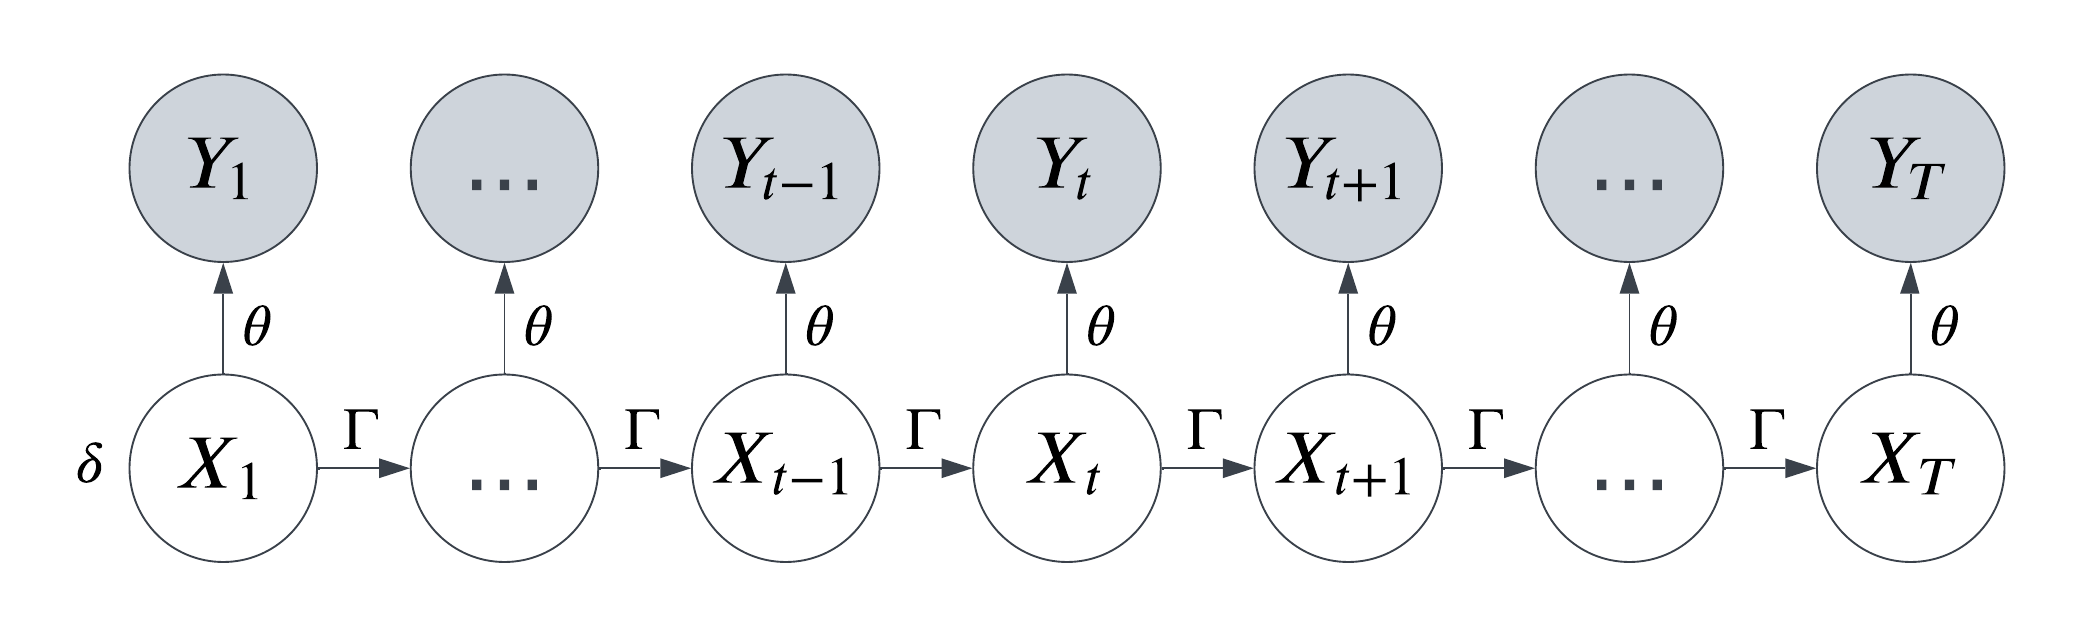
\includegraphics[width=5in]{../plt/HMM.png}
    \caption{Graphical representation of an HMM. $X_t$ corresponds to an unobserved latent state at time $t$ whose distribution is described by a Markov chain. $Y_t$ corresponds to an observation at time $t$, where $Y_t$ given all other observations $\bfY \setminus \{Y_t\}$ and hidden states $\bfX$ depends only on $X_t$.}
    \label{fig:HMM}
\end{figure}

For brevity, we denote the full set of parameters as $\bfphi \equiv \{\bftheta,\bfeta\}$. We also denote the set of parameter associated with the initial distribution as $\bfeta^{(\cdot)} = \{\eta^{(i)}\}_{i=1}^N$, and the set of parameters associated with the transition probability matrix as $\bfeta^{(\cdot,\cdot)} = \{\eta^{(i,j)}\}_{i,j=1}^N$. 

The joint likelihood of an HMM given observations $\bfY$ and latent states $\bfX$ is
%
\begin{equation}
    p(\bfX,\bfY;\bfphi) = \delta^{(X_1)} f^{(X_1)}(Y_1; \theta^{(X_1)}) \prod_{t=2}^T \Gamma^{(X_{t-1},X_t)} f^{(X_t)}(Y_t; \theta^{(X_t)}).
    \label{eqn:like}
\end{equation}
%
Alternatively, the marginal likelihood of the observed data $\bfY$ alone is 
%
\begin{equation}
    p(\bfY;\bfphi) = \delta P(Y_1;\bftheta) \prod_{t=2}^T \bfGamma P(Y_t;\bftheta) \mathbf{1}_N,
    \label{eqn:like_marginal}
\end{equation}
%
where $\mathbf{1}_N$ is an $N$-dimensional column vector of ones and $P(y_t;\bftheta)$ is an $N \times N$ diagonal matrix with entry $(i,i)$ equal to $f^{(i)}(y_t; \theta^{(i)})$. For a more complete introduction to HMMs, see \citet{Zucchini:2016}.
%
\subsection{State Decoding}
%
%GET RID OF FUNCTIONS IN BACKGROUND SECTION
%
%ADD FUNCTIONS (TILDES) RIGHT BEFORE ALG 4 AND MAKE TILDE FUNCTION ARGUMENTS NOT ALPHA t-1, and then comment that putting in $\alpha_t-1(\bfphi)$ gives the right value
%
%SAY THAT WE ASSUME PHI IS FIXED
%
%CHANGE GRADIENT ESTIMATES TO GRADIENT APPROXIMATIONS???
%
%ADD HATS TO ALPHAS, BETAS, ETC
%
%CHANGE WORDING FOR GRADIENTS TO APPROXIMATIONS
%
% MAKE ALL PARAMETERS BOLDED
%
One appealing feature of HMMs is that it is simple to determine the distribution of a given hidden state ($X_t$) conditioned on the set of observations $\bfY$. Assuming that the HMM parameters $\bfphi$ are fixed, define the probability density of the observations between times $s$ and $t$ as $p(Y_{s:t};\bfphi)$. Likewise, define \textit{forward probabilities} $\alpha^{(i)}_t = p(y_{1:t},X_t = i;\bfphi)$ (for $i = 1,\ldots,N$ and $t = 1,\ldots,T$) and \textit{backward probabilities} $\beta^{(i)}_t = p(y_{(t+1):T}|X_t = i;\bfphi)$ (for $i = 1,\ldots,N$ and $t = 1,\ldots,T-1$). By convention, $\beta^{(i)}_T = 1$ for $i = 1,\ldots,N$. Both $\alpha_t$ and $\beta_t$ can be calculated using the following recursion: % We define the mapping from $\alpha_{t-1}(\bfphi)$ and $\bfphi$ to $\alpha_t(\bfphi)$ as $\tilde \alpha_t(\alpha_{t-1}(\bfphi),\bfphi)$. However, $\alpha_t(\bfphi)$ itself is a function of $\bfphi$ alone, which we denote as $\alpha_t$. Similarly, we define the mapping from $\beta_{t+1}(\bfphi)$ and $\bfphi$ to $\beta_{t}(\bfphi)$ as $\tilde \beta_t(\alpha_{t+1}(\bfphi),\bfphi)$ and the mapping from only $\bfphi$ to $\beta_t$ as $\beta_t(\bfphi)$. 

\begin{align}
    \alpha_1^{(i)}(\bfphi) = \tilde \alpha_1^{(i)}(\bfphi) \quad &= \quad  \delta^{(i)} ~ f^{(i)} ~ (y_1;\theta^{(i)}), \label{eqn:alpha_1} \\
    %
    \alpha_t^{(i)}(\bfphi) = \tilde \alpha_t^{(i)}(\alpha_{t-1}(\bfphi),\bfphi) \quad &= \quad \sum_{j=1}^N ~ \alpha_{t-1}^{(j)}(\bfphi) ~ \Gamma^{(j,i)} ~ f^{(i)}(y_t;\theta^{(i)}), \quad t = 2,\ldots,T, \label{eqn:alpha} \\
    %
    \beta_T^{(i)}(\bfphi) = \tilde \beta_T^{(i)}(\bfphi) \quad &= \quad  1, \label{eqn:beta_T} \\
    %
    \beta_t^{(i)}(\bfphi) = \tilde \beta_t^{(i)}(\beta_{t+1}(\bfphi), \bfphi) \quad &= \quad \sum_{j=1}^N ~ \Gamma^{(i,j)} ~ f^{(j)}(y_{t+1};\bftheta) ~ \beta^{(j)}_{t+1}(\bfphi), \quad t = 1,\ldots,T-1. \label{eqn:beta}
\end{align}
%
%It is important to note that $\alpha_t$ and $\beta_t$ are functions of $\bfphi$ alone. We nonetheless abuse notation and write $\alpha_t$ and $\beta_t$ as functions of $\alpha_{t-1}$ and $\beta_{t+1}$ as well to illustrate the recursion. In addition, it takes $\calO(N^2)$ time to calculate $\alpha_{t}$ and $\beta_{t}$ if $\alpha_{t-1}$, $\beta_{t+1}$, and $\bfphi$ are known. However, it takes $\calO(TN^2)$ time to calculate $\alpha_{t}$ and $\beta_{t}$ if only $\bfphi$ is known, as the recursions starting from $\alpha_1$ and $\beta_T$ must be performed.
%
Note that it takes $\calO(N^2)$ time to evaluate $\tilde \alpha_t (\alpha_{t-1},\bfphi)$ and $\tilde \beta_t(\beta_{t+1},\bfphi)$, but $\calO(TN^2)$ time to evaluate $\alpha_t(\bfphi)$ and $\beta_t(\bfphi)$. In future sections we abuse notation and write $\alpha_t(\bfphi)$ and $\beta_t(\bfphi)$ as $\alpha_t$ and $\beta_t$ for brevity. 

We denote the probability that $X_t = i$ given all observations $\bfY$ and parameters $\bfphi$ as $\gamma_t^{(i)}(\bfphi)$ for $t = 1,\ldots,T$ and $i = 1,\ldots,N$. Further, we denote the probability that $X_{t-1} = i$ and $X_t = j$ given all observations $\bfY$ and parameters $\bfphi$ as $\xi_t^{(i,j)}(\bfphi)$ for $t = 2,\ldots,T$ and $i,j = 1,\ldots,N$. Namely,

\begin{gather}
    \gamma_t^{(i)}(\bfphi) = \bbP(X_t = i \mid \bfY ~;~ \bfphi), \\ \xi_t^{(i,j)}(\bfphi) = \bbP(X_{t-1} = i, X_t = j \mid \bfY ~;~ \bfphi).
\end{gather}
%
Both $\gamma_t$ and $\xi_t$ can be calculated from $\alpha_{t-1}$, $\alpha_t$, $\beta_t$, and $\bfphi$ using the following mappings:

\begin{align}
    \gamma_t^{(i)}(\bfphi) = \tilde \gamma_{t}^{(i)}(\alpha_t,\beta_t) \quad &= \quad   \frac{\alpha_{t}^{(i)} ~ \beta_{t}^{(i)}}{\sum_{i'} \alpha_{t}^{(i')} ~ \beta_{t}^{(i')}}, \label{eqn:gamma} \\
    %
    \xi_{t}^{(i,j)}(\bfphi) = \tilde \xi_{t}^{(i,j)}(\alpha_{t-1},\beta_{t},\bfphi) \quad &= \quad \frac{\alpha_{t-1}^{(i)} ~ \Gamma^{(i,j)} ~ f^{(j)}(y_{t} ~ ; ~\bftheta) ~ \beta_{t}^{(j)}}{\sum_{i',j'} ~ \alpha_{t-1}^{(i')} ~ \Gamma^{(i',j')} ~ f^{(j')}(y_{t} ~ ; ~\bftheta) ~ \beta_{t}^{(j')}} \label{eqn:xi}.
\end{align}
%
It takes $\calO(N^2)$ time to evaluate $\tilde \gamma_{t}(\alpha_t,\beta_t)$ and $\tilde \xi_{t}^{(i,j)}(\alpha_{t-1},\beta_{t},\bfphi)$, but $\calO(TN^2)$ time to evaluate $\gamma_t(\bfphi)$ and $\xi_t(\bfphi)$. %In future sections we abuse notation and write $\gamma_t(\bfphi)$ and $\xi_t(\bfphi)$ as $\gamma_t$ and $\xi_t$ for brevity. 

\subsection{The Baum-Welch Algorithm}

The Baum-Welch algorithm is a specific instance of the EM algorithm used to estimate the parameters of the HMM. %Suppose a sequence of observations $\bfY$ is observed as output of a latent-variable model with unknown latent states $\bfX$ and unknown parameters $\bfphi$.
At iteration $k$ of the EM algorithm, denote the current parameter estimates as $\bfphi_{k}$. One iteration of the EM algorithm consists of an expectation (or E) step, followed by a maximization (or M) step. For the E step, the function $Q(\bfphi \mid \bfphi_{k})$ is defined as the expected value of the joint log-likelihood $\log p(\bfY,\bfX; \bfphi)$ when $\bfX$ is a random variable with density $p(\bfX \mid \bfY ; \bfphi_{k})$. For the M step, the next parameter estimate $\bfphi_{k+1}$ is found by maximizing $Q(\bfphi \mid \bfphi_{k})$ with respect to the parameters $\bfphi$:
%
\begin{gather}
    Q(\bfphi \mid \bfphi_{k}) \equiv \bbE_{\bfphi_{k}}\left[\log p(\bfY,\bfX;\bfphi) \mid \bfY \right] \label{eqn:Q} \\
    %
    %Q^*(\bfphi_{k}) \equiv \max_{\bfphi}Q(\bfphi \mid \bfphi_{k})\\
    %
    \bfphi_{k+1} = \argmax_{\bfphi} Q(\bfphi \mid \bfphi_{k}). \label{eqn:BW_update}
\end{gather}
%
Combining Equation (\ref{eqn:Q}) with Equation (\ref{eqn:like}) and performing some algebra yields the following expression for $Q$: %separate the expected value into three convenient terms:
\begin{equation}
    Q(\bfphi \mid \bfphi_{k}) %&\equiv \bbE_{\bfphi_{k}}\left[\log p(\bfY,\bfX;\bfphi) \mid \bfY \right] \\
    %
    %&= \bbE_{\bfphi_{k}} \left[\sum_{t=1}^T \log f^{(X_t)}(y_t;\theta^{(X_t)}) + \log \delta^{(X_1)} + \sum_{t=2}^{T} \log \Gamma^{(X_{t-1},X_{t})} \mid \bfY \right] \\
    %
    %&= \sum_{t = 1}^T \bbE_{\bfphi_{k}} \left[ \log f^{(X_t)}(y_t;\theta^{(X_t)}) \mid \bfY \right]  \\
    %& \qquad + \bbE_{\bfphi_{k}} \Big[\log \delta_{X_1} \mid \bfY \Big] + \sum_{t=2}^{T} \bbE_{\bfphi_{k}} \left[ \log \Gamma^{(X_{t-1},X_{t})} \mid \bfY \right] \\
    %
    = \sum_{t = 1}^T \sum_{i=1}^N \gamma^{(i)}_t(\bfphi_{k}) \log f^{(i)}(y_t;\theta^{(i)}) + \sum_{i=1}^N \gamma^{(i)}_1(\bfphi_{k}) \log \delta^{(i)} + \sum_{t=2}^{T} \sum_{i=1}^N \sum_{j=1}^N \xi_t^{(i,j)}(\bfphi_{k}) \log \Gamma^{(i,j)}
    \label{eqn:Q_sum}
\end{equation}
%The first term and last two terms on the right-hand side of the equation above only depend upon $\theta$ and $\eta$, respectively. The maximization problem in Equation (\ref{eqn:BW_update}) can thus be divided into two separate sub-problems as follows. Note that we define the objective functions $F$ and $G$ below so that the M step of the EM algorithm is a minimization problem consistent with existing optimization literature.
%
%\begin{gather}
%    F_t^{(k)}(\bftheta) \equiv F_t(\theta, \bfphi_{k}) \equiv - \sum_{i=1}^N \gamma^{(i)}_t(\bfphi_{k}) \log f^{(i)}(y_t;\theta^{(i)}), \\
    %
%    F^{(k)}(\bftheta) \equiv F(\theta, \bfphi_{k}) \equiv \frac{1}{T} \sum_{t=1}^T F^{(k)}_t(\bftheta), \label{eqn:F} \\
    %
%    \theta_{k+1} = \argmin_{\theta} F^{(k)}(\bftheta), \label{eqn:EM_update_theta} \\ \nonumber \\
    %
    %
%    G_1^{(k)}(\eta) \equiv G_1(\eta, \bfphi_{k}) \equiv - \sum_{i=1}^N \gamma^{(i)}_1(\bfphi_{k})\log \delta^{(i)}(\eta) \\
    %
%    G_t^{(k)}(\eta) \equiv G_t(\eta, \bfphi_{k}) \equiv - \sum_{i=1}^N \sum_{j=1}^N \xi^{(i,j)}_t(\bfphi_{k}) \log \Gamma^{(i,j)}(\eta), \quad t \geq 2 \\
    %
%    G^{(k)}(\eta) \equiv G(\eta, \bfphi_{k}) = \frac{1}{T} \sum_{t=1}^{T} G_t(\eta, \bfphi_{k}), \label{eqn:G}\\
    %
%    \eta_{k+1} = \argmin_{\eta} G(\eta,\bfphi_{k}). \label{eqn:EM_update_eta}
%\end{gather}
%In addition, note that 
%\begin{equation}
%   Q(\bfphi \mid \bfphi_{k}) = -T ~ \left[F(\theta, \bfphi_{k}) + G(\eta, \bfphi_{k})\right].
%\end{equation}
%
More detailed pseudocode for the E and the M step are given in Algorithms (\ref{alg:E}) and (\ref{alg:EM}).
%
\begin{algorithm}
\caption{\texttt{E-step}($\bfphi_k$)}\label{alg:E}
\begin{algorithmic}[1]
\Require Parameter value $\bfphi_k$.
%
\State $\alpha_1 \gets \tilde \alpha_1(\bfphi_k)$
\State $\beta_T \gets \tilde \beta_T(\bfphi_k)$
\For{$t = 2,\ldots,T$}
    \State $\alpha_t \gets \tilde \alpha_t(\alpha_{t-1},\bfphi_k)$
    \State $\beta_{T+1-t} \gets \tilde \beta_t(\beta_{T+2-t},\bfphi_k)$
\EndFor
%
\State $\gamma_1 \gets \tilde \gamma_1(\alpha_{1},\beta_{1})$
\For{$t = 2,\ldots,T$}
    \State $\gamma_t \gets \tilde \gamma_t(\alpha_{t},\beta_{t})$
    \State $\xi_t \gets \tilde \xi_t(\alpha_{t-1},\beta_{t},\bfphi_{k})$
\EndFor
%
\State \Return $\{\alpha,\beta,\gamma,\xi\}$
\end{algorithmic}
\end{algorithm}
%
%
%
\begin{algorithm}
\caption{\texttt{Baum-Welch}$(\bfphi_0,K)$}\label{alg:EM}
\begin{algorithmic}[1]
\Require Initial parameter values $\bfphi_0$, number of iterations $K$
\For{$k = 0,\ldots,K-1$}
    \State $\{\alpha,\beta,\gamma,\xi\} \gets \texttt{E-step}(\bfphi_{k})$ \Comment{E step} 
    \State \Comment{M step} $$\bfphi_{k+1} \gets \argmax_{\{\bftheta,\bfeta\}} \sum_{t = 1}^T \sum_{i=1}^N \gamma^{(i)}_t \log f^{(i)}(y_t;\theta^{(i)}) + \sum_{i=1}^N \gamma^{(i)}_1 \log \delta^{(i)}(\eta) + \sum_{t=2}^{T} \sum_{i=1}^N \sum_{j=1}^N \xi_t^{(i,j)} \log \Gamma^{(i,j)}(\eta)$$
\EndFor
\State \Return $\bfphi_K$
\end{algorithmic}
\end{algorithm}
%
In many simple scenarios the maximization problem in Equation (\ref{eqn:BW_update}) above has a closed-form solution. For example, if $\bfGamma$ does not depend upon any covariates and $f^{(i)}(y_t;\theta^{(i)})$ is a normal or Poisson probability density function with respect to $y_t$, then the solution of Equation (\ref{eqn:BW_update}) is given in Section 4.2 of \citet{Zucchini:2016}. However, in many other situations the maximization problem above is not straightforward and requires numerical maximization techniques. %For example, finding closed-form solutions to the M step for the HHMM defined in section \ref{subsec:HHMM} is not straightforward. 
We thus review different methods for numerical maximization via stochastic optimization. %We describe several such scenarios in the subsequent section. 

\subsection{Stochastic Optimization}
\label{subsec:stoch_optim}

Stochastic optimization techniques are used to solve minimization problems where the objective function is a sum of many terms \citep{Robbins:1951}. %In much of the stochastic optimization literature, this optimization problem takes the form of a minimization over an average:
Namely,
%
\begin{equation}
    \bfphi^* = \argmin_{\bfphi} F(\bfphi), \qquad F(\bfphi) = \frac{1}{T}\sum_{t = 1}^T F_t(\bfphi).
    \label{eqn:stoch_opt}
\end{equation}
%

%Within the M step of the $k^{th}$ iteration of the EM algorithm, 
Standard gradient descent at a given step $m$ with step size $\lambda$ updates the parameter value $\bfphi_{m}$ by moving in the direction of the negative gradient of $F$. The step size $\lambda$ is a user-defined value that should large enough to allow the algorithm to move quickly to a minimum of $F$, but not so large that $\bfphi_m$ ``overshoots" the minimum. Formally, the update step is written as
%
\begin{equation}
    \bfphi_{m+1} = \bfphi_{m} - \lambda \nabla F(\bfphi_{m}) =  \bfphi_{m} - \frac{\lambda}{T} \sum_{t=1}^T \nabla F_t(\bfphi_{m}).
\end{equation}
%
However, this update requires evaluating a gradient for all $t = 1,\ldots,T$, which can be prohibitively expensive if $T$ is large. In contrast, stochastic gradient descent (SGD) updates $\bfphi$ using an unbiased estimate of the full gradient \citep{Robbins:1951}:
%
\begin{equation}
    \bfphi_{m+1} = \bfphi_{m} - \lambda \nabla F_{t_{m}}(\bfphi_{m})
\end{equation}
%
for some $t_{m} \in \{1,\ldots,T\}$ selected uniformly at random at step $m$ of the algorithm. Stochastic gradient descent reduces the amount of time between updates by using an unbiased estimate of the gradient to update $\bfphi_{m}$. However, the gradient estimates themselves can have high variance, so stochastic gradient descent requires that the step size $\lambda$ decays over time to ensure convergence. In addition, SGD has slower convergence rates compared to full gradient descent \citep{Schmidt:2017}.

Variance-reduced stochastic optimization techniques such as stochastic average gradient descent (SAG) \citep{Schmidt:2017}, stochastic variance reduced gradient descent (SVRG) \citep{Johnson:2013}, and SAGA \citep{Defazio:2014} enjoy the speed of stochastic gradient descent as well as the convergence rates of full gradient descent. These algorithms involve gradient estimates $\widehat \nabla F_t$ whose average approximates the full gradient $\nabla F(\bfphi_{m})$. The gradient estimates are updated at various stages in the optimization algorithm and are used to reduce the variance of full gradient estimate. 
%In particular, SAG uses the update rule:
%
%\begin{equation}
%    \bfphi_{m+1} \gets \bfphi_{m} - \lambda \left[\frac{\nabla F^{(k)}_{t_m}(\bfphi_{m}) - \widehat \nabla F^{(k)}_{t_m}}{T} + \frac{1}{T} \sum_{t=1}^T \widehat \nabla F^{(k)}_{t} \right], \label{eqn:SAG_update}
%\end{equation}
%
%which is simply the table average with entry $t_m$ updated at step $m$. This update rule is intuitive, but it represents a biased estimate of the gradient $\nabla P(\bfphi_m)$. This can slow down convergence and makes theoretical analysis of SAG difficult. 
For example, SVRG and SAGA update $\bfphi$ using an unbiased estimate of the gradient:
%
\begin{equation}
    \bfphi_{m+1} = \bfphi_{m} - \lambda \left[\nabla F_{t_{m}}(\bfphi_{m}) - \widehat \nabla F_{t_{m}} + \widehat \nabla F \right],
    \label{eqn:SAGA_update}
\end{equation}
%
where
%
\begin{equation}
    \widehat \nabla F = \frac{1}{T} \sum_{t=1}^T \widehat \nabla F_{t}.
    \label{eqn:tbl_avg}
\end{equation}
%Taking the expected value of the gradient estimate from (\ref{eqn:SAGA_update}) shows that it is unbiased:
%
%\begin{align}
%    \bbE\left[\nabla F^{(k)}_{t_m}(\bfphi_{m}) - \widehat \nabla F^{(k)}_{t_m} + \frac{1}{T} \sum_{t=1}^T \widehat \nabla F^{(k)}_{t} \right] &= \frac{1}{T} \sum_{t=1}^T \nabla F^{(k)}_{t}(\bfphi_{m}) - \frac{1}{T} \sum_{t=1}^T \widehat \nabla F^{(k)}_{t} + \frac{1}{T} \sum_{t=1}^T \widehat \nabla F^{(k)}_{t} \\
    %
%    &= \frac{1}{T} \sum_{t=1}^T \nabla F^{(k)}_{t_m}(\bfphi_{m}) = \nabla F^{(k)}(\bfphi_{m}).
%\end{align}
%
After updating the parameters at step $m$, SAGA simply updates the table average and the table of gradients at position $t_{m}$.
%
%\begin{gather}
%    \widehat \nabla F \gets \widehat \nabla F + \frac{1}{T} \nabla F_{t_{m}}(\bfphi_{m}) - \frac{1}{T} \widehat \nabla F_{t_{m}}, \\
    %
%    \widehat \nabla F_{t_{m}} \gets \nabla F_{t_{m}}(\bfphi_{m}).
%\end{gather}
%
%After updating the table at position $t_m$ with the SAG/SAGA update rule, the table average $\frac{1}{T} \sum_{t=1}^T \widehat \nabla F^{(k)}_{t}$ must be updated using the previous estimate of $\widehat \nabla F^{(k)}_{t}$. 
%
%This trade-off should be considered by practitioners when deciding between the two algorithms. 
%
Algorithm (\ref{alg:VRSO}) outlines SVRG and SAGA in pseudocode. SAGA involves running the algorithm until convergence, but the gradient estimates $\widehat \nabla F_t$ are never updated when using SVRG within Algorithm (\ref{alg:VRSO}). As such, SVRG involves repeatedly running Algorithm (\ref{alg:VRSO}) with $M \propto T$ so that the table of gradient estimates remains up-to-date.

\begin{algorithm}
\caption{\texttt{VRSO}$(F,\bfphi_0,\lambda,A,M)$}\label{alg:VRSO}
\begin{algorithmic}[1]
\Require Loss function $F = \frac{1}{T}\sum_{t=1}^T F_t$, initial value $\bfphi_0$, step size $\lambda$, algorithm $A \in \{\text{SVRG, SAGA}\}$, and number of iterations $M$.
%
\vspace{5pt}
\For{$t = 1,\ldots,T$} \Comment{initialize gradients and table average}
\State $\widehat \nabla F_t \leftarrow \nabla F_t (\bfphi_0)$
\EndFor
\State $\widehat \nabla F \gets \frac{1}{T} \sum_{t=1}^T \widehat \nabla F_{t}$
%
\For{$m = 0,\ldots,M-1$}:
    %
    \State Pick $t_{m} \in \{1,\ldots,T\}$ uniformly at random.
    %
    \State \Comment{update parameters}
    \begin{gather}
        \bfphi_{m+1} = \bfphi_{m} - \lambda \left[\nabla F_{t_m}(\bfphi_{m}) - \widehat \nabla F_{t_{m}} + \widehat \nabla F \right]
        \label{eqn:SAGA_update0}
    \end{gather}
    %
    \If{$A$ = SAGA}:
    \Comment{update table average and table at index $t_{m}$}
        \begin{gather}
            \widehat \nabla F \gets \widehat \nabla F + \frac{1}{T} \left( \nabla F_{t_m}(\bfphi_{m}) - \widehat \nabla F_{t_{m}}\right), \\
            \widehat \nabla F_{t_{m}} \gets \nabla F_{t_m}(\bfphi_{m}).
        \end{gather}
    \EndIf
\EndFor
\State \Return $\bfphi_M$
\end{algorithmic}
\end{algorithm}


%Whether or not Equations (\ref{eqn:EM_update_theta}) and (\ref{eqn:EM_update_eta}) have closed-form solutions, even defining $F^{(k)}$ and $G^{(k)}$ to initialize the optimization problem (the E-step) has a time cost of $\calO(T)$, which can be expensive for large $T$. 


%%%%%%%%%%%%


\subsection{Variations of Hidden Markov Models}
\label{subsec:HHMM}

Hidden Markov models rely on several assumptions that are often violated in real-world applications. For example, high-frequency data often violates the assumption that the underlying state process of an HMM is time-homogeneous %, and that the observations are independent when conditioned on the hidden state process 
\citep{Sidrow:2021}. As such, researchers have introduced several variations, such as incorporating covariates into the transition probability matrix $\Gamma$ to account for changing dynamics in the transition matrix \citep{McClintock:2018}. In addition, if a sequence of observations displays multi-scale dependence structure, then it may be more appropriate to use a \textit{hierarchical} hidden Markov model, or HHMM \citep{Barajas:2017,Adam:2019,Sidrow:2021}. Hierarchical HMMs are useful because they capture dependence structures of the hidden process on multiple time scales. There are many different particular ways to define a Hierarchical HMM, such as the formulations in \citet{Barajas:2017}, \citet{Adam:2019}, and \citet{Sidrow:2021}. As presented here, Hierarchical HMMs involve some coarse-scale hidden process that evolves over time. While the coarse-scale state remains in the same state, a fine-scale hidden process evolves simultaneously. Observations are then generated according to a distribution that depends jointly on both the hidden coarse-scale state and the hidden fine-scale state. However, once the coarse-scale process changes states, the fine-scale process restarts and evolves depending upon that new coarse-scale state.

The parameters of an HHMM are defined to enforce this hierarchical structure for the hidden Markov chain. In particular, define a coarse-scale Markov chain $\{X^{(c)}_t\}_{t=1}^T$ parameterized by a pre-determined number of coarse-scale hidden states $N^{(c)} \in \bbN$, a coarse-scale initial distribution $\delta^{(c)} \in \bbR^{N^{(c)}}$ and coarse-scale probability transition matrix $\boldsymbol{\Gamma}^{(c)} \in \bbR^{{N^{(c)}} \times {N^{(c)}}}$. For each coarse-scale state $i$, we yet define another fine-scale Markov chain with states $X^{(f)}_t$ whose length is randomly determined by the dwell time of the coarse-scale Markov chain in state $i$. The $i^{th}$ fine-scale Markov chain is parameterized by a pre-determined number of fine-scale states $N^{(f,i)} \in \bbN$. It also has initial distribution $\delta^{(f,i)} \in \bbR^{N^{(f,i)}}$, and a fine-scale transition probability matrix $\boldsymbol{\Gamma}^{(f,i)} \in \bbR^{N^{(f,i)} \times N^{(f,i)}}$. In summary, 
%
\begin{gather}
    \delta^{(c,i)} = \bbP\left( X_1^{(c)} = i \right) \qquad 
    \Gamma^{(c,i,j)} = \bbP\left( X_{t+1}^{(c)} = j | X_{t}^{(c)} = i \right) \\
    %
    \delta^{(f,i,i')} = \bbP\left( X_{t+1}^{(f)} = i' | X_{t}^{(c)} \neq i, X_{t+1}^{(c)} = i \right) \qquad 
    \Gamma^{(f,i,i',j')} = \bbP\left( X_{t+1}^{(f)} = j' | X_{t}^{(f)} = i', X_{t}^{(c)} = i, X_{t+1}^{(c)} = i \right).
\end{gather}
%
Define the matrix $\boldsymbol{\Pi}^{(f,i)}$ as an $N^{(f,i)} \times N^{(f,i)}$ matrix with identical row entries $\delta^{(f,i)}$. Using this parameterization, the set of pairs $\{(X^{(c)}_t,X^{(f)}_t)\}_{t=1}^T$ is itself Markov chain. It has a total of $N \equiv \sum_{i=1}^{N^{(c)}} N^{(f,i)}$ hidden states, a global initial distribution of
%
\begin{equation} 
\boldsymbol{\delta} = 
\begin{pmatrix}
\delta^{(c,1)}\boldsymbol{\delta}^{(f,1)} & \delta^{(c,2)}\boldsymbol{\delta}^{(f,2)}    & \cdots & \delta^{(c,N^{(c)})}\boldsymbol{\delta}^{(f,N^{(c)})}
\end{pmatrix},
\label{eqn:global_delta}
\end{equation}
%
and a global probability transition matrix of %\textcolor{red}{I stole this from Vianey}:
%
\begin{equation} 
\boldsymbol{\Gamma} = 
\begin{pmatrix}
\Gamma^{(c,1,1)}\boldsymbol{\Gamma}^{(f,1)}     & \Gamma^{(c,1,2)} \boldsymbol{\Pi}^{(f,2)}     & \cdots & \Gamma^{(c,1,N^{(c)})}\boldsymbol{\Pi}^{(f,N^{(c)})}  \cr
\Gamma^{(c,2,1)}\boldsymbol{\Pi}^{(f,1)} & \Gamma^{(c,2,2)} \boldsymbol{\Gamma}^{(f,2)}  & \cdots & \Gamma^{(c,2,N^{(c)})}\boldsymbol{\Pi}^{(f,N^{(c)})} \cr
\vdots & \vdots & \ddots & \vdots \cr 
\Gamma^{(c,N^{(c)},1)}\boldsymbol{\Pi}^{(f,1)} & \Gamma^{(c,N^{(c)},2)}\boldsymbol{\Pi}^{(f,2)}      & \cdots & \Gamma^{(c,N^{(c)},N^{(c)})} \boldsymbol{\Gamma}^{(f,N^{(c)})} 
\end{pmatrix}.
\label{exptpm2}
\end{equation}
%
%corresponds to the probability that the initial coarse-scale hidden state is $i$, and $\Gamma^{(c,i,j)}$ corresponds to the probability that the coarse-scale hidden state will transition to coarse-scale state $j$ given that the current coarse-scale state is $i$. Further, $\delta^{(f,i,i')}$ corresponds to the probability that the initial fine-scale hidden state is $i'$ after transitioning to state $i$ from another state. Finally, $\Gamma^{(f,i,i',j')}$ corresponds to the probability that the fine-scale hidden state will transition to state $j'$ given that the current coarse-scale state is $i$ and the current fine-scale state is $i'$.
%
%Namely, $\delta^{(c,i)} = \bbP\left(X_1^{(c)}\right)$ corresponds to the probability that the initial coarse-scale hidden state is $i$, and $\Gamma^{(c,i,j)}$ corresponds to the probability that the coarse-scale hidden state will transition to coarse-scale state $j$ given that the current coarse-scale state is $i$. Further, $\delta^{(f,i,i')}$ corresponds to the probability that the initial fine-scale hidden state is $i'$ after transitioning to state $i$ from another state. Finally, $\Gamma^{(f,i,i',j')}$ corresponds to the probability that the fine-scale hidden state will transition to state $j'$ given that the current coarse-scale state is $i$ and the current fine-scale state is $i'$.
%
The transition probability matrix $\boldsymbol{\Gamma}$ and initial distribution $\boldsymbol{\delta}$ of a hierarchical HMM is simply a more restricted version of the same parameters for a standard HMM. A visualization of a hierarchical Markov chain with $N^{(c)} = 2$ and $N^{(f,1)} = N^{(f,2)} = 2$ is shown in Figure (\ref{fig:HHMM}).
%
\begin{figure}
    \centering
    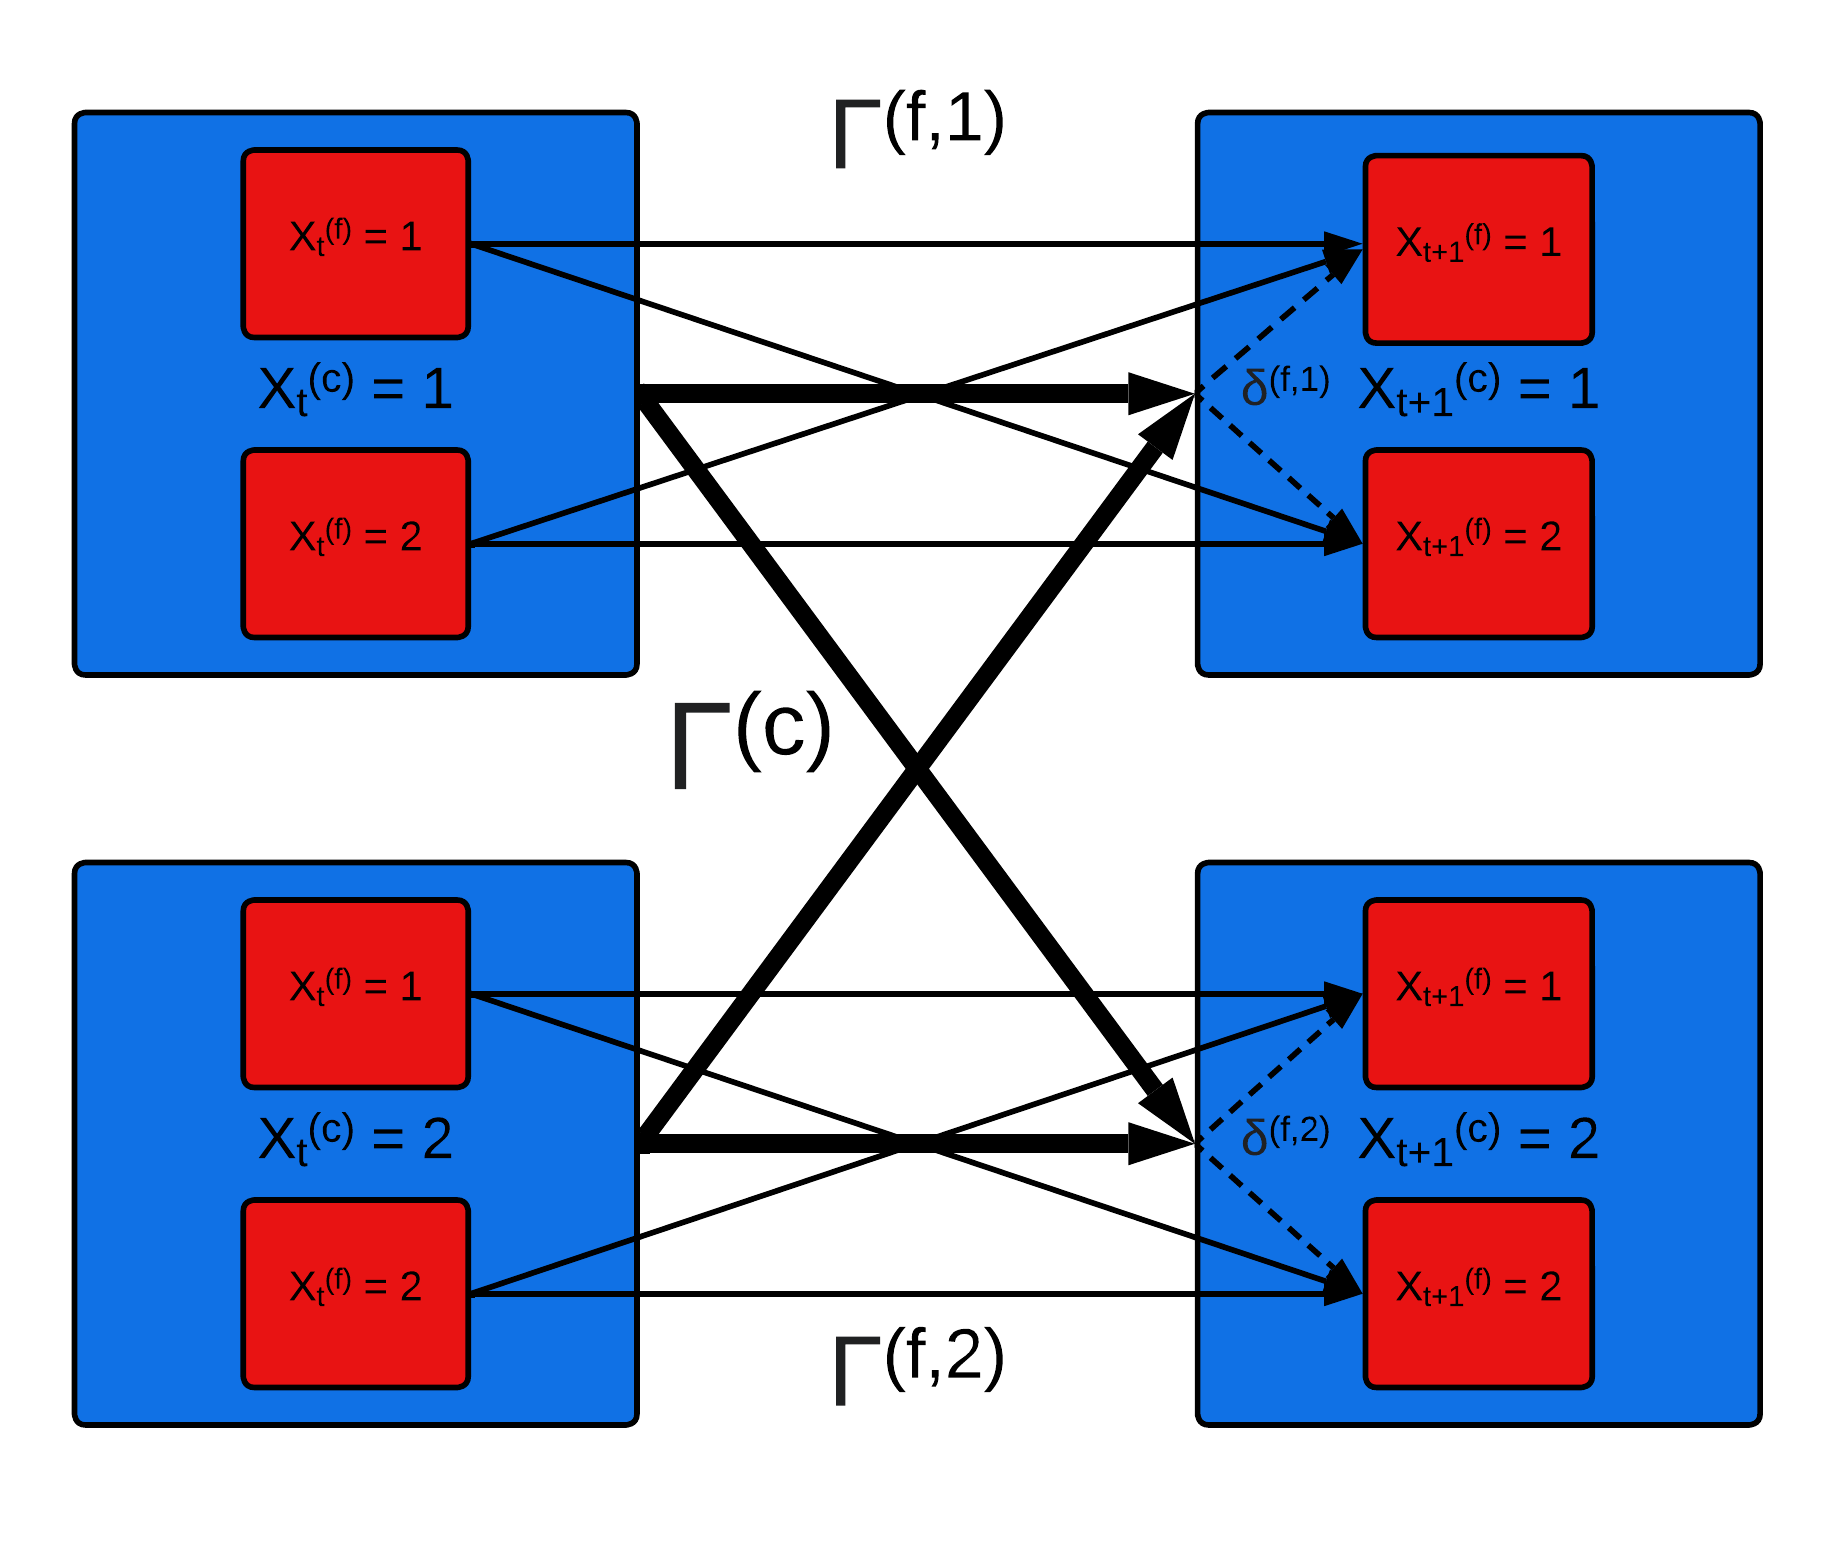
\includegraphics{plt/HHMM.png}
    \caption{Visualization of the underlying Markov chain for a hierarchical HMM with $N^{(c)} = 2$ and $N^{(f,1)} = N^{(f,2)} = 2$. Solid thick lines correspond to entries of $\boldsymbol{\Gamma}^{(c)}$. Solid thin lines correspond to entries of $\boldsymbol{\Gamma}^{(f,i)}$ for $i = 1,2$, which describes the distribution of $X_{t+1}^{(f)}$ if $X^{(c)}_{t} = X^{(c)}_{t+1} = i$. Dashed thin lines correspond to entries of $\boldsymbol{\delta}^{(f,i)}$ for $i = 1,2$, which describes the distribution of $X_{t+1}^{(f)}$ if $X^{(c)}_{t} \neq X^{(c)}_{t+1} = i$.}
    \label{fig:HHMM}
\end{figure}

The coarse-scale and fine-scale initial distributions and transition probability matrices are parameterized similarly to Equation (\ref{eqn:reparam}). In particular, $\boldsymbol{\Gamma}^{(c)}$ and $\boldsymbol{\delta}^{(c)}$ are parameterized via $\eta^{(c)}$ as follows:
%
\begin{equation}
    \Gamma^{(c,i,j)}(\eta^{(c)}) = \frac{\exp(\eta^{(c,i,j)})}{\sum_{k=1}^N \exp(\eta^{(c,i,k)})}, \qquad \delta^{(c,i)}(\eta^{(c)}) = \frac{\exp(\eta^{(c,i)})}{\sum_{k=1}^N \exp(\eta^{(c,k)})}
    \label{eqn:reparam_coarse}
\end{equation}
%
Likewise, $\boldsymbol{\Gamma}^{(f,i)}$ and $\delta^{(f,i)}$ are parameterized via $\eta^f$ as follows:
%
\begin{equation}
    \Gamma^{(f,i,i',j')}(\eta^f) = \frac{\exp(\eta^{(f,i,i',j')})}{\sum_{k'=1}^N \exp(\eta^{(f,i,i',k')})}, \qquad \delta^{(f,i,i')}(\eta^{f}) = \frac{\exp(\eta^{(f,i,i')})}{\sum_{k'=1}^N \exp(\eta^{(f,i,k')})}.
    \label{eqn:reparam_fine}
\end{equation}


\begin{algorithm}
\begin{algorithmic}
\If{$\nabla_{\phi} Q^{(k)}(\phi_{k}) < \epsilon$}:
    \State return $\phi_{k}$
\EndIf

\If{using version 1 and $\log p(\bfy;\phi_{k,\ell+1}) \geq \log p(\bfy;\phi_{k})$}:
    \Comment{move to next iteration}
    \State $\phi_{k+1} \gets \phi_{k,\ell}$
    \State $k \gets k+1$
    \State return to step 2
\ElsIf{using version 2 and $Q^*(\phi_{k}) - Q\big(\phi_{k,\ell} ~ \big| ~ \phi_{k}\big) \leq \frac{\zeta + 1}{2} \Big(Q^*(\phi_{k}) - Q \big(\phi_{k} ~ \big| ~ \phi_{k}\big) \Big)$}
    \State $\phi_{k+1} \gets \phi_{k,\ell,M}$
    \State $k \gets k+1$
    \State return to step 2
\Else
    \State $\ell \gets \ell+1$
    \State return to step 4
\EndIf

\end{algorithmic}
\end{algorithm}

\section{Outline of alternative proof}

Here we give an outline for a proof that for all $\delta > 0$ and all $\epsilon > 0$, $\lim_{k \to \infty} \bbP(||\nabla L (\bfphi_k) || > \delta) < \epsilon$.

\begin{enumerate}
    \item By way of contradiction, assume that for some $\delta > 0$ and $\epsilon > 0$, for all $K$ there exists some $k > K$ such that $\bbP \left(||\nabla \log p(\bfphi_k)|| > \delta \right) > \epsilon$.
    %
    \item Note that $\log p(\bfphi_k)\overset{p}{\to} \log p^*$ for some $\log p^*$ by the monotone convergence theorem since the map strictly increases the likelihood, and the likelihood is bounded (by assumption).
    %
    \item By definition of convergence in probability, for the $\delta > 0$ and $\epsilon > 0$ from step 1, there exists some $K$ such that for all $k > K$:
    $$\bbP\left(|\log p(\bfphi_{k}) - \log p^*| > \frac{\delta^2(1-\zeta)}{8L}\right) < \frac{1-\zeta}{2}\epsilon$$
    %
    \item Pick the $k > K$ such that $\bbP \left(||\nabla \log p(\bfphi_k)|| > \delta \right) > \epsilon$. Create a lower bound on the probability above applied to $\bfphi_{k+1}$:
    %
    \begin{align*}
        &\bbP\left(|\log p(\bfphi_{k+1}) - \log p^*| > \frac{\delta^2(1-\zeta)}{8L}\right) \\ 
        %
        &\geq \bbP\Big(|\log p(\bfphi_{k+1}) - \log p^*| > \frac{\delta^2(1-\zeta)}{8L}, |\log p(\bfphi_k) - \log p^*| < \frac{\delta^2(1-\zeta)}{8L}, ||\nabla \log p(\bfphi_k)|| > \delta \Big) \\
        %
        &= \bbP\Big(|\log p(\bfphi_{k+1}) - \log p^*| > \frac{\delta^2(1-\zeta)}{8L} \Big| |\log p(\bfphi_k) - \log p^*| < \frac{\delta^2(1-\zeta)}{8L}, ||\nabla \log p(\bfphi_k)|| > \delta \Big) \\
        %
        & * \bbP\left( |\log p(\bfphi_k) - \log p^*| < \frac{\delta^2(1-\zeta)}{8L}, ||\nabla \log p(\bfphi_k)|| > \delta \right) \\ 
        %
        & > \bbP\Big(|\log p(\bfphi_{k+1}) - \log p^*| > \frac{\delta^2(1-\zeta)}{8L} \Big| |\log p(\bfphi_k) - \log p^*| < \frac{\delta^2(1-\zeta)}{8L}, ||\nabla \log p(\bfphi_k)|| > \delta \Big) \\
        %
        & * \bbP \left(||\nabla \log p(\bfphi_k)|| \geq \delta \right) - \bbP\left( |\log p(\bfphi_k) - \log p^*| > \frac{\delta^2(1-\zeta)}{8L}\right) \\
        %
        & \geq \bbP\Big(|\log p(\bfphi_{k+1}) - \log p^*| > \frac{\delta^2(1-\zeta)}{8L} \Big| |\log p(\bfphi_k) - \log p^*| < \frac{\delta^2(1-\zeta)}{8L}, ||\nabla \log p(\bfphi_k)|| > \delta \Big) * (\epsilon - \epsilon(\frac{1-\zeta}{2})) \\
        %
        & = \bbP\Big(|\log p(\bfphi_{k+1}) - \log p^*| > \frac{\delta^2(1-\zeta)}{8L} \Big| |\log p(\bfphi_k) - \log p^*| < \frac{\delta^2(1-\zeta)}{8L}, ||\nabla \log p(\bfphi_k)|| > \delta \Big) * \epsilon(\frac{1+\zeta}{2})
    \end{align*}
    %
    \item Now focus on the long conditional probability, and denote it as $\bbP_k$. Start with Markov's inequality for the SVRG condition:
    %
    $$\bbP_k\left[Q_{\bfphi_k}(\bfphi^*_{k+1}) - Q_{\bfphi_k}(\bfphi_{k+1}) < \frac{1+\zeta}{2}\left(Q_{\bfphi_k}(\bfphi^*_{k+1}) - Q_{\bfphi_k}(\bfphi_{k})\right)\right] > \frac{1-\zeta}{1+\zeta},$$
    %
    and do some algebra with two assumptions: $Q_{\bfphi_k}(\bfphi^*_{k+1}) \geq Q_{\bfphi_k}(\bfphi_k) + \frac{\delta^2}{2L}$, and $\log p(\bfphi_{k+1}) - \log p(\bfphi_{k}) > Q_{\bfphi_k}(\bfphi_{k+1}) - Q_{\bfphi_k}(\bfphi_{k})$. Then we get to
    %
    \begin{align*}
        \bbP_k\left[Q_{\bfphi_k}(\bfphi^*_{k+1}) - Q_{\bfphi_k}(\bfphi_{k+1}) < \frac{1+\zeta}{2}\left(Q_{\bfphi_k}(\bfphi^*_{k+1}) - Q_{\bfphi_k}(\bfphi_{k})\right)\right] &> \frac{1-\zeta}{1+\zeta} \\
        %
        \bbP_k\left[- Q_{\bfphi_k}(\bfphi_{k+1}) < \left(1-\frac{1+\zeta}{2}\right)\left(-Q_{\bfphi_k}(\bfphi^*_{k+1})\right) + \left(\frac{1+\zeta}{2}\right) \left(-Q_{\bfphi_{k}}(\bfphi_{k})\right)\right] &> \frac{1-\zeta}{1+\zeta} \\
        %
        \bbP_k\left[-Q_{\bfphi_k}(\bfphi_{k+1}) < \left(1-\frac{1+\zeta}{2}\right)\left(-Q_{\bfphi_k}(\bfphi_{k}) - \frac{\delta^2}{2L}\right) + \left(\frac{1+\zeta}{2}\right) \left(-Q_{\bfphi_{k}}(\bfphi_{k})\right) \right] &> \frac{1-\zeta}{1+\zeta} \\
        %
        \bbP_k\left[-Q_{\bfphi_k}(\bfphi_{k+1}) < -Q_{\bfphi_k}(\bfphi_{k}) - \left(\frac{\delta^2(1-\zeta)}{4L}\right) \right] &> \frac{1-\zeta}{1+\zeta} \\
        %
        \bbP_k\left[Q_{\bfphi_k}(\bfphi_{k+1}) - Q_{\bfphi_k}(\bfphi_{k}) >  \left(\frac{\delta^2(1-\zeta)}{4L}\right) \right] &> \frac{1-\zeta}{1+\zeta} \\
        %
        \bbP_k\left[\log p(\bfphi_{k+1}) - \log p(\bfphi_{k}) >  \left(\frac{\delta^2(1-\zeta)}{4L}\right) \right] &> \frac{1-\zeta}{1+\zeta} \\
        %
        \bbP_k\left[|\log p(\bfphi_{k+1}) -\log p^*| + |\log p^* - \log p(\bfphi_{k})| >  \left(\frac{\delta^2(1-\zeta)}{4L}\right) \right] &> \frac{1-\zeta}{1+\zeta} \\
        %
        \bbP_k\left[|\log p(\bfphi_{k+1}) -\log p^*| + \left(\frac{\delta^2(1-\zeta)}{8L}\right) >  \left(\frac{\delta^2(1-\zeta)}{4L}\right) \right] &> \frac{1-\zeta}{1+\zeta} \\
        %
        \bbP_k\left[|\log p(\bfphi_{k+1}) - \log p^*| >  \left(\frac{\delta^2(1-\zeta)}{8L}\right) \right] &> \frac{1-\zeta}{1+\zeta}
    \end{align*}
    %
    \item This leaves the following inequality:
    \begin{equation}
        \bbP\left[|\log p(\bfphi_{k+1}) - \log p^*| > \frac{\delta^2(1-\zeta)}{8L} \right] > (\frac{1-\zeta}{1+\zeta})(\frac{1+\zeta}{2})\epsilon = \frac{1-\zeta}{2} \epsilon \label{eqn:eps_2}
    \end{equation}
    %
    However, this a contradiction since we assumed the exact opposite in step 3.
\end{enumerate}

Since $\delta > 0$ and $\epsilon$ was arbitrary, and we know that $\log p(\bfphi_k) \overset{p}{\to} \log p^*$ by the monotone convergence theorem, we know that $\log p(\bfphi_k)$ converges to $\log p(\bfphi^*)$, and $||\nabla \log p(\bfphi_k)|| \overset{p}{\to}||\nabla \log p(\bfphi^*)|| = 0$